\documentclass[12pt,a4paper]{report}
\usepackage{pgfplots}
\usepackage{amsmath}
\usepackage{graphicx}
\usepackage{fancyhdr}
\usepackage{tikz}
\usepackage{multirow}
\usepackage{booktabs}
\usepackage{makecell}

\makeatletter
\renewcommand{\@chapapp}{Week}
\makeatother

\pgfplotsset{compat=1.18}

\title{Fundamental Labs\\DC Motor Manufacture and Control}
\author{Prabhnoor Singh Sahni}
\date{\today}

\begin{document}

\maketitle
\tableofcontents

\chapter{Brushed Motor}
\section{Bipolar Motor Building}
In this section we will be building a DC motor. We begin by collecting the required parts as given to us in the manual.
Then we make the encoder board by soldering the parts. Then we carefully cut pieces of the metal sheet to make the brush of the motor and finally we assemble the motor. After making sure that all the four brushes are properly touching the motor and the connections are not loose. We try to rotate the motor and we see that everything works.
\section{Rotational Speed Measurement}
First we make a semicircular disk and connect it to the motor, this will pass through the photointerrupter and will make it possible to determine the speed as we shall see later.
Now we will connect the DC Motor Control Board to our setup. This board will measure the number of times the disk is crossing the photointerrupter and give us the number of rotations of the motor in 0.42 seconds. We confirm the operation of the board. \\
Now we also connect our oscilloscope to the circuit and set up our system for final measurement. We rotate the motor and begin taking measurements from oscilloscope as well as from the DC motor control board. \\
For the oscilloscope we set the time interval to 200 ms and measure the rpm.
When we set our voltage to 15V, we look at the square waves on the oscilloscope and record the data. We measure the time interval and number of rotations. For 15V, we have 606.6 ms and 935.8 ms which gives us \[\frac{(935.8-606.6)\text{ ms}}{4}=12.2\text{ rotations/s}=729\text{ rpm}.\]
We repeat this for 3 different voltage values corresponding to low (15V), medium (17V) and high (18V) and the results are in 
Table~\ref{tab:volt_rpm}.\\
For 17V, \[\frac{(516.2-437.6)\text{ ms}}{1}=763.4\text{ rpm},\]
for 18V, \begin{equation}\frac{(1041-924)ms}{1} = 1025\text{ rpm}\end{equation}
Then we count the number of rotations from the DC motor control board. On this board, we need to see the lights that are ON, which indicate 1 in binary. The steps are again repeated for the three voltages as in Table~\ref{tab:volt_rpm}. \\

\begin{table}[ht]
    \centering
    \caption{Revolutions per minute (rpm) measured from motor control board and oscilloscope at different voltages}
    \label{tab:volt_rpm}
    \begin{tabular}{|cc|c|c|c|}
        \hline
	    & & \multicolumn{3}{c|}{\textbf{Voltage}} \\
        \cline{3-5}
	    & & \textbf{Small (15V)} & \textbf{Medium (17V)} & \textbf{High (18V)} \\
        \hline
	    \multirow{2}{*}{\textbf{rpm}} & \multicolumn{1}{|c|}{Motor Control Board} & 1000 rpm & 1571 rpm  & 1714 rpm \\
	    \cline{2-5}
	    & \multicolumn{1}{|c|}{Oscilloscope} & 729 rpm  & 763.4 rpm & 1025 rpm \\
        \hline
    \end{tabular}
\end{table}

If we look at Table~\ref{tab:volt_rpm}, we can see stark difference in the rpm measured from the oscilloscope and board. It is possible that the motor control board is inaccurate because it only takes into account integer values and this can cause discrepancies in our data. 
Now, in order to analyse our brushed motor a bit further, we need to look at the speed of the motor using brush timing adjustment. In our DC motor, we have brushes which need to make contact with the motor and change the direction of electric current in rotations. The timing of the brushes refers to the precise moment when the brushes switch the electrical current to different segments of the commutator and  reverses the direction of current flow in the rotor windings and maintains continuous rotation. We aim to change this timing and see how the speed changes. To adjust the timing we change the position of the rotor notches, we loosen the screw and change the position of rotor notches with respect to a horizontal line. We do this for 5 different angles as in Table~\ref{tab:angle_rot}.

\begin{table}[ht]
	\centering
	\caption{Revolutions per minute corresponsing to different positions of the rotor notch by adjusting angles}
	\label{tab:angle_rot}
	\begin{tabular}{|c|c|}
		\hline
		Angle & RPM \\
		\hline
		\(0^{\circ}\) & 2285.7 \\
		\hline
		\(45^{\circ}\) & 2000 \\
		\hline
		\(90^{\circ}\) & 0 \\
		\hline
		\(135^{\circ}\) & 0 \\
		\hline
		\(180^{\circ}\) & -2285.7\\
		\hline
	\end{tabular}
\end{table}

We can see in this table (Table~\ref{tab:angle_rot}) that we have maximum rpm of the motor at 0 degrees and 180 degrees (although the motor rotates in opposite direction). This angle is when the brushes are aligned with the neutral axis of the armature coil. \\

\begin{figure}[ht]
	\centering
	\includegraphics[width=\textwidth]{figures/brush_dc.pdf}
	\caption{The four stages of rotation for a brushed DC motor}
	\label{fig:brush_dc}
\end{figure}

\subsection{Assignment K1,K2}
\subsubsection{K1\ Brushed direct current motor}
\begin{enumerate}
	\item \textbf{Why brushed DC motors rotate and what is the role of brushes?}\\
		Let's look at Figure~\ref{fig:brush_dc} which depicts the different stages of motor rotation. 
		If we look at the first stage, the brush on the left touching the armature coil is in contact with the positive terminal and the 
		brush on the other side is in contact with the negative terminal. Thus, current flows from left to right. 
		Due to this a magnetic field is generated in the coil, which points to the left (from right hand rule). 
		At this stage we can also see that the magnet is in such a position that the South pole of the magnet is close to the left coil 
		and the north pole is close to the right coil. In such a scenario, we see from the figure that like poles are near each other, 
		this would cause them to repel. 
		Thus, there is a 90 degrees rotation in the clockwise direction and we get to the situation of the second stage.\\ 
		Here, we can see that since our motor moved 90 degrees, 
		the north pole is now near the left coil and south pole is near the right coil. Also look at the armature coil, we see that the 
		coil has rotated; however, due to the structure of the metal sheet on the coil, the left brush is still in contact with the 
		positive terminal and the right brush with the negative terminal. 
		This maintains the direction of current and in turn the direction of poles on the coils. Thus, in this stage the north pole that 
		has now reached the left coil is near the south pole and the south pole of the magnet that has reached the right coil is near the 
		north pole. Opposite poles are now near each other! They will now attract, making the motor rotate in the same direction another 
		90 degrees. See Figure~\ref{fig:brush_dc}.\\
		After a total 180 degree rotation, the third stage is a complete opposite of the first stage. The magnet's north pole is near the 
		left coil and south pole near the right. The armature coil has again rotated and now the left brush has come in contact with the 
		negative terminal and right brush has come in contact with the positive terminal. This flips the direction of current. Since the 
		direction of current has changed, the current going into the coil will be in different direction, this will cause the magnetic 
		field produced to flip its direction as well. Thus, the coil's poles will flip. The north pole is now on the right and the south 
		pole on the left. And due to this, the north pole of the magnet is near the north pole of the coil and the south pole of the 
		magnet is near the south pole of the coil. This will again cause them to repel and they will again rotate another 90 degrees in 
		clockwise direction. We see that even though the poles of the magnet are opposite, the rotation of the armature coil coupled with the 
		flipping of current direction makes the rotation continue. \\
		Finally, we move to stage 4, when the armature coil, the magnet and the motor as a whole have completed three quarters of rotation in the same 
		direction. 
		In this stage, the poles of the magnet are, north pole near the right coil and south pole near the left coil. Now, even after rotation of the 
		armature coil, it is still connected to the same terminals and the direction of current remains the same, just like we saw in the second stage. 
		So, in this stage the direction of current is from right to left and therefore the poles of the coil are the same. Looking at Figure~\ref{fig:brush_dc} we again see that opposite poles are near each other and they will attract. This will make the motor rotate another 90 degrees and thereby completing a full 360 degree rotation. This process continues for the motor's rotation. \\
		We saw in this process how important the role of brushes was. Basically brushes play in role in reversing the direction of current after every half a rotation. 
		Whenever, after a rotation of 180 degrees, the part of the armature coil that was connected to the left brush and the part that was connected to the right brush reverses its connection. Now they get connected to opposite brushes, making current direction change and in turn make magnetic field of coil change, thus making sure that motor rotation direction remains consistent. If the direction of current is not reversed by brushes the motor will rotate backwards i.e. after half a rotation clockwise it will do another half rotation anti-clockwise. It will be a to-and-fro rotation where the motor comes back after every 180 degrees. \\
	\item \textbf{Positional Relationship of rotor and magnets}\\
		Looking at Table~\ref{tab:angle_rot} we can understand the we get can get highest rpm from motor only when at the starting position, 
		the angle is at 0 degrees or 180 degrees (for 180 degrees, direction of motor is opposite). At this angle, the coil and brushes are 
		oriented in the neutral position. At this angle the armature coil winding is perpendicular to the magnetic field lines. 
\end{enumerate}

\subsubsection{K2\ Enter the rotational speed Measurement results.}
\begin{enumerate}
	\item We have recorded the data in Table~\ref{tab:volt_rpm}. The rotational speed that was determined from the oscilloscope seems more accurate compared to the one determined from the DC motor control board. The reason is that the oscilloscope is able to count complete cycles and we can see the square waves on the screen. On the other hand, the board counts every time the fan/disk crosses the photointerrupter, it counts each rotation very fast. Moreover, the rotations it counts are per 0.42 seconds which is a very small duration. Further, board counts the rotations in binary representing values 0 to \text{16} in  numbers. The board does not take into account decimal digits. It cannot count in decimal, only counts integers. Lastly, there is a higher possibility of human error while counting from the board. This is because lights blink and it becomes hard to accurately determine the speed. Hence, the oscilloscope is more accurate. \\
	\item In order to improve the accuracy of the motor control board we can do a number of things. Firstly, we can configure the board to measure rotations for long time. Currently the board measures rotations per 0.42 seconds. However, if we increase this time interval then the accuracy can be increased. \\
		Another way to improve the accuracy is to change the shape of the disk. Currently we're using a semicircular disk. If we change the shape to something like fan with two quarters of the 
		disk cut on the diagonals. In this way after every 90 degree rotation the output of the photointerrupter would change because if for first 90 degrees there is some part of the disk, then 
		after that there will be no disk part and then after another 90 degrees there will be the second disk part and in the last 90 degrees there will be the hollow part 
		and then it would continue rotating like that. This will help improve accuracy of counting because our control board counts in very short intervals. 
\end{enumerate}

\chapter{Brushless DC Motor}
\section{Velocity Characteristics Measurement}
We begin by removing the brush (making sure that the four brushes are not touching the armature coil of the motor). 
Then we make some changes in the circuit, to make a brushless DC motor. We configure the motor circuit according to the circuit given in 
Figure~\ref{fig:brushless_dc}. 
The new connections made help in changing the direction of voltage output to the motor according to changes in signals from the encoder which sends 
signals based on detection from photointerrupter.
\begin{figure}[ht]
	\includegraphics[width=\textwidth]{figures/brushless_dc.png}
	\caption{Connection of motor, DC motor control board, and power supply}
	\label{fig:brushless_dc}
\end{figure}

\begin{table}[ht]
	\centering
	\caption{Relationship between light shielding plate position and voltage at terminals A and B}
	\label{tab:light_shield}
	\begin{tabular}{|c|c|c|c|}
		\hline
		{Light Shielding Plate} & A [V] & B [V] & Direction of Voltage\\
		\hline
		Present & \({783.8\times 10^{-3}}\) & 3.385 & B$\rightarrow$ A \\
		\hline
		Not Present & 3.385 & ${783.8 10^{-3}}$ & A$\rightarrow$ B\\
		\hline
	\end{tabular}
\end{table}
\subsection{Assignment K3}
\begin{enumerate}
	\item After making the connections, we connect the different terminals to observe the wave characteristics on the oscilloscope and see the 
		voltage.
		We find how there are differences in voltages when a light shielding plate exists or not. We also check the characteristics at both 
		terminals A and B. The data is recorded in Table~\ref{tab:light_shield}. 
	\item The light shielding plate plays a crucial role in changing the direction of voltage. This makes the motor rotate. It is very crucial.
	\item There are many reasons why a brushless motor is more effective compared to a brushed motor. 
		\begin{itemize}
			\item There is no friction due to brushes in a brushless motor. This makes rotation smooth and without any constraint. 
			\item The connection between motor and brush doesn't matter. In the case of brushed motor, it is important that the brushes 
				are touching the motor at all times. If this connection is not proper then there may be some problems. 
			\item In the case of brushed motor there are sparks or shorting on the brushes. This is not good. On the other hand, there 
				is no such shorting in brushless motor. 
			\item In the case of brushless motor there is no heat loss from the system. Thus energy is not wasted, this makes the 
				brushless motor more efficient than brushed motor.
		\end{itemize}
\end{enumerate}
Now we make adjustments to our system so that the straight-line part of the semicircular disk is perpendicular to the floor surface when in this state. 
The orientation of this disk with the motor plays a crucial role in determing motor rotation characteristics. We see that on making this adjustment our motor begins to rotate. \\
Next we check rotation of motor at different alignment of the semicircular disk. We consider the present position as 0 degrees and get the rotation data for -90 degrees, -45 degrees, 0 degrees, 45 degrees and 90 degrees in Table~\ref{tab:rpm_angles}.
\subsection{Assignment K4}
\begin{enumerate}
	\item Using the data obtained from our experiments we draw a graph for rpm values of the different angles as in Figure~\ref{fig:rpm_angles}. 
		We can see that the RPM value is maximum for the case when angle of orientation of the semicircular disk is 90 degrees. 
\begin{figure}[h]
\centering
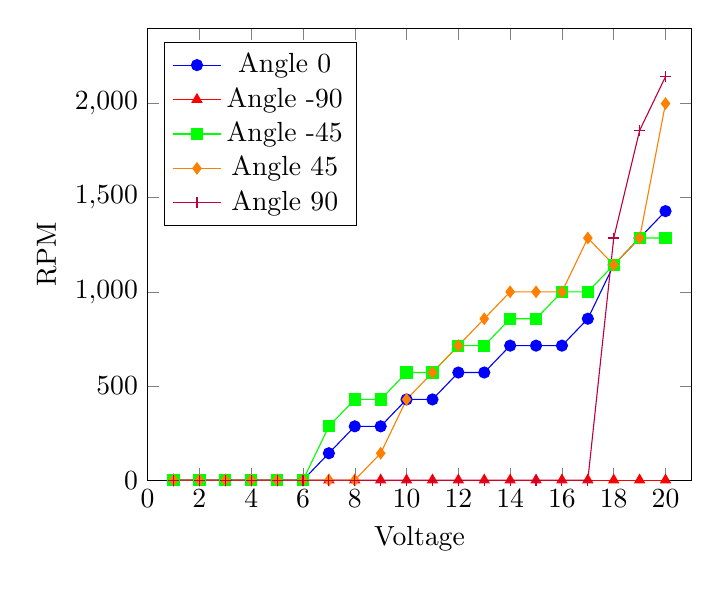
\begin{tikzpicture}
\begin{axis}[
    width=.7\textwidth,
    xlabel={Voltage},
    ylabel={RPM},
    xmin=0, xmax=21,
    ymin=0, ymax=2400,
    xtick={0,2,4,6,8,10,12,14,16,18,20},
    ytick={0,500,1000,1500,2000},
    legend pos=north west,
    grid style=dashed,
]

\addplot[color=blue, mark=*] coordinates {
(1,0) (2,0) (3,0) (4,0) (5,0) (6,0) (7,142.8571429) (8,285.7142857) (9,285.7142857) (10,428.5714286) (11,428.5714286) (12,571.4285714) (13,571.4285714) (14,714.2857143) (15,714.2857143) (16,714.2857143) (17,857.1428571) (18,1142.857143) (19,1285.714286) (20,1428.571429)
};

\addplot[color=red, mark=triangle*] coordinates {
(1,0) (2,0) (3,0) (4,0) (5,0) (6,0) (7,0) (8,0) (9,0) (10,0) (11,0) (12,0) (13,0) (14,0) (15,0) (16,0) (17,0) (18,0) (19,0) (20,0)
};

\addplot[color=green, mark=square*] coordinates {
(1,0) (2,0) (3,0) (4,0) (5,0) (6,0) (7,285.7142857) (8,428.5714286) (9,428.5714286) (10,571.4285714) (11,571.4285714) (12,714.2857143) (13,714.2857143) (14,857.1428571) (15,857.1428571) (16,1000) (17,1000) (18,1142.857143) (19,1285.714286) (20,1285.714286)
};

\addplot[color=orange, mark=diamond*] coordinates {
(1,0) (2,0) (3,0) (4,0) (5,0) (6,0) (7,0) (8,0) (9,142.8571429) (10,428.5714286) (11,571.4285714) (12,714.2857143) (13,857.1428571) (14,1000) (15,1000) (16,1000) (17,1285.714286) (18,1142.857143) (19,1285.714286) (20,2000)
};

\addplot[color=purple, mark=+] coordinates {
(1,0) (2,0) (3,0) (4,0) (5,0) (6,0) (7,0) (8,0) (9,0) (10,0) (11,0) (12,0) (13,0) (14,0) (15,0) (16,0) (17,0) (18,1285.714286) (19,1857.142857) (20,2142.857143)
};

\legend{Angle 0, Angle -90, Angle -45, Angle 45, Angle 90}
\end{axis}
\end{tikzpicture}
\caption{RPM Values for Different Angles of orientation of the semicircular disk for a brushless DC motor}\label{fig:rpm_angles}
\end{figure}

\item Since for our brushless DC motor the frequency of rotation is very high, therefore, we can approximate the square wave for the rotations to a sine wave as follows:
	Consider \[V=V_0Sin(\omega t).\]
	Due to the inductor coil there will be a self induced emf because current in coil is changing which causes a change in electric field (time varying electric field generates emf, we know this by Faraday's Law)\\ But \[V+V_L=0,\] where \(V_L\) is induced emf. 
		\begin{align}
			-L \frac{dI}{dt} &= V_L\\
			-L \frac{dI}{dt} + V_0Sin(\omega t) &= 0\\
			L\int{dI}&=\int{V_0Sin(\omega t)dt}\\
			LI&=-\frac{V_0}{\omega}Cos(\omega t)\\
			I(t)&=\frac{V_0}{\omega L}Sin(\omega t-\frac{\pi}{2})
\end{align}
Thus we can see that in the case of a brushless DC motor the current lags the voltage by 90 degrees. So, in order to compensate for this
delay in current the light shielding plate is set to 90 degrees, this helps
in compensating the delay of current and we get maximum rpm.
\item No the optimal rotor angle of brushed motor did not equal the angle of the light shielding plate at which the rotationsal speed was at its maximum. 
	The frequency of a brushless DC motor is very high so we can approximate the square waves to sine waves. 
	In a brushed DC motor we saw that the current was changing direction every half a rotation and the maximum rpm was achieved when the angle of orientation was 0 degrees. 
But for a brushless motor, we see that 90 degrees is maximum, but why? The reason is that since current lags the voltage by 90 degrees we need to compensate that lag. 
This is why when the orientation is 90 degrees in a brushless motor, the exact same situation as when the angles is 0 degrees in brushed DC motor is achieved. This ensures maximum rpm. 
\end{enumerate}

\begin{table}[htbp]
\centering
\caption{Revolutions per Minute of the brushless motor for Different Angles of the Light Shielding Plate}\label{tab:rpm_angles}
\begin{tabular}{|c|c|c|c|c|c|}
\hline
 & \multicolumn{5}{c|}{\textbf{Revolutions per Minute}} \\ \hline
	\textbf{Voltage} & Angle 0 & Angle -90 & Angle -45 & Angle 45 & Angle 90 \\ \hline
1  & 0 & 0 & 0 & 0 & 0 \\
2  & 0 & 0 & 0 & 0 & 0 \\
3  & 0 & 0 & 0 & 0 & 0 \\
4  & 0 & 0 & 0 & 0 & 0 \\
5  & 0 & 0 & 0 & 0 & 0 \\
6  & 0 & 0 & 0 & 0 & 285.7142857 \\
7  & 142.8571429 & 0 & 285.7142857 & 0 & 571.4285714 \\
8  & 285.7142857 & 0 & 428.5714286 & 0 & 857.1428571 \\
9  & 285.7142857 & 0 & 428.5714286 & 142.8571429 & 1000 \\
10 & 428.5714286 & 0 & 571.4285714 & 428.5714286 & 1000 \\
11 & 428.5714286 & 0 & 571.4285714 & 571.4285714 & 1000 \\
12 & 571.4285714 & 0 & 714.2857143 & 714.2857143 & 1000 \\
13 & 571.4285714 & 0 & 714.2857143 & 857.1428571 & 1000 \\
14 & 714.2857143 & 0 & 857.1428571 & 1000 & 1000 \\
15 & 714.2857143 & 0 & 857.1428571 & 1000 & 1000 \\
16 & 714.2857143 & 0 & 1000 & 1000 & 1000 \\
17 & 857.1428571 & 0 & 1000 & 1285.714286 & 1000 \\
18 & 1142.857143 & 0 & 1142.857143 & 1142.857143 & 1285.714286 \\
19 & 1285.714286 & 0 & 1285.714286 & 1285.714286 & 1857.142857 \\
20 & 1428.571429 & 0 & 1285.714286 & 2000 & 2142.857143 \\
\hline
\end{tabular}
\end{table}


\section{Feedback Based Control System Configuration}%
In this section we make some changes to the wiring to add a feedback loop to our motor. 
We aim to understand Rotational Speed Control for a brushless DC motor using Feedback through these experiments. 
\subsection{Assignment K5}
\begin{enumerate}
	\item I have checked and confirmed that the voltage supplied from the power supply output terminals changes when the values shown by the LED change. 
	\item In this experiment we recorded the data for RPM corresponding to when the voltage is falling from HIGH to LOW in Table~\ref{tab:rpm_voltage_high_to_low} and the data 
		corresponding to RPM for when the voltage is rising from LOW to HIGH in Table~\ref{tab:rpm_voltage_low_to_high}. For this data, we recorded the values in every 10 seconds. 
	\item Next, we plot our data for both the cases on a graph. 
		Figure~\ref{fig:rpm_time} represents the relationship of revolutions per minute with time 
		for both cases and Figure~\ref{fig:voltage_time} represents the relationship of voltage with time. 
		We can see the trend of the graph and we understand the HIGH and LOW values for our system. 
\end{enumerate}

\begin{table}[htbp]
\centering
\caption{RPM versus Voltage (Low to High)}\label{tab:rpm_voltage_low_to_high}
\begin{tabular}{cccc}
\toprule
	\textbf{Voltage [V]} & \textbf{Time [s]} & \makecell[c]{\textbf{Revolutions per}\\\textbf{0.42 seconds}} & \textbf{RPM (Low to High)} \\
\midrule
7     & 0    & 2  & 285.7142857 \\
8     & 10   & 3  & 428.5714286 \\
8.5   & 20   & 4  & 571.4285714 \\
9     & 30   & 5  & 714.2857143 \\
9.5   & 40   & 6  & 857.1428571 \\
10    & 50   & 7  & 1000 \\
10.5  & 60   & 7  & 1000 \\
11    & 70   & 8  & 1142.857143 \\
11.5  & 80   & 8  & 1142.857143 \\
12    & 90   & 8  & 1142.857143 \\
12.5  & 100  & 8  & 1142.857143 \\
12.5  & 110  & 8  & 1142.857143 \\
12.5  & 120  & 8  & 1142.857143 \\
12.5  & 130  & 8  & 1142.857143 \\
12.5  & 140  & 8  & 1142.857143 \\
12.5  & 150  & 8  & 1142.857143 \\
12.5  & 160  & 8  & 1142.857143 \\
12.5  & 170  & 8  & 1142.857143 \\
12.5  & 180  & 8  & 1142.857143 \\
12.5  & 190  & 8  & 1142.857143 \\
\bottomrule
\end{tabular}
\end{table}


\begin{table}[htbp]
\centering
\caption{RPM versus Voltage (High to Low)}\label{tab:rpm_voltage_high_to_low}
\begin{tabular}{cccc}
\toprule
	\textbf{Voltage [V]} & \textbf{Time [s]} & \makecell[c]{\textbf{Revolutions per}\\\textbf{0.42 seconds}} & \textbf{RPM (High to Low)} \\
\midrule
10    & 0    & 9  & 1285.714286 \\
9     & 10   & 8  & 1142.857143 \\
8.5   & 20   & 7  & 1000 \\
8     & 30   & 6  & 857.1428571 \\
10.5  & 40   & 5  & 714.2857143 \\
7     & 50   & 5  & 714.2857143 \\
7     & 60   & 5  & 714.2857143 \\
7     & 70   & 5  & 714.2857143 \\
7     & 80   & 5  & 714.2857143 \\
7     & 90   & 5  & 714.2857143 \\
7     & 100  & 5  & 714.2857143 \\
7     & 110  & 5  & 714.2857143 \\
7     & 120  & 5  & 714.2857143 \\
7     & 130  & 5  & 714.2857143 \\
7     & 140  & 5  & 714.2857143 \\
7     & 150  & 5  & 714.2857143 \\
7     & 160  & 5  & 714.2857143 \\
7     & 170  & 5  & 714.2857143 \\
7     & 180  & 5  & 714.2857143 \\
7     & 190  & 5  & 714.2857143 \\
\bottomrule
\end{tabular}
\end{table}


\begin{figure}[htbp]
\centering
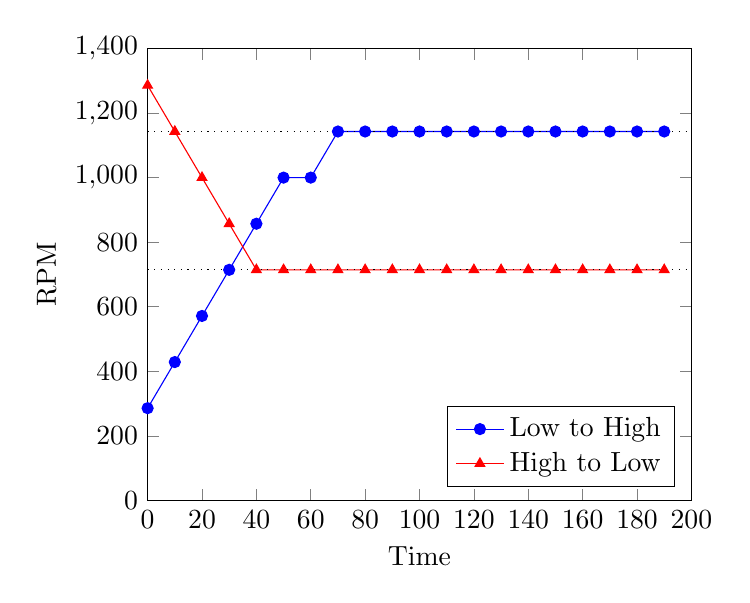
\begin{tikzpicture}
\begin{axis}[
    width=.7\textwidth,
    xlabel={Time},
    ylabel={RPM},
    xmin=0, xmax=200,
    ymin=0, ymax=1400,
    xtick={0,20,40,60,80,100,120,140,160,180,200},
    ytick={0,200,400,600,800,1000,1200,1400},
    legend pos=south east, % Adjust the legend position here
    grid style=dashed,
]

% Low to high data
\addplot[color=blue, mark=*] coordinates {
(0,285.7142857) (10,428.5714286) (20,571.4285714) (30,714.2857143) (40,857.1428571) (50,1000) (60,1000) (70,1142.857143) (80,1142.857143) (90,1142.857143) (100,1142.857143) (110,1142.857143) (120,1142.857143) (130,1142.857143) (140,1142.857143) (150,1142.857143) (160,1142.857143) (170,1142.857143) (180,1142.857143) (190,1142.857143)
};

% High to low data
\addplot[color=red, mark=triangle*] coordinates {
(0,1285.714286) (10,1142.857143) (20,1000) (30,857.1428571) (40,714.2857143) (50,714.2857143) (60,714.2857143) (70,714.2857143) (80,714.2857143) (90,714.2857143) (100,714.2857143) (110,714.2857143) (120,714.2857143) (130,714.2857143) (140,714.2857143) (150,714.2857143) (160,714.2857143) (170,714.2857143) (180,714.2857143) (190,714.2857143)
};

\draw[dotted] (0,1142.857143) -- (200,1142.857143);
\draw[dotted] (0,714.2857143) -- (200,714.2857143);

\legend{Low to High, High to Low}
\end{axis}
\end{tikzpicture}
	\caption{Plot illustrating relationship between Revolutions per minute and Time for when the voltage is rising (LOW to HIGH) and falling (HIGH to LOW)}\label{fig:rpm_time}
\end{figure}

\begin{figure}[htbp]
\centering
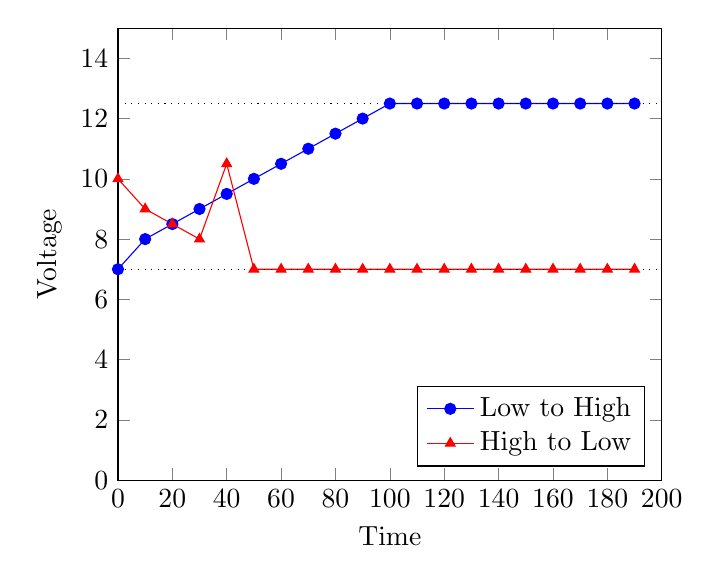
\begin{tikzpicture}
\begin{axis}[
    width=.7\textwidth,
    xlabel={Time},
    ylabel={Voltage},
    xmin=0, xmax=200,
    ymin=0, ymax=15,
    xtick={0,20,40,60,80,100,120,140,160,180,200},
    ytick={0,2,4,6,8,10,12,14},
    legend pos=south east, % Adjust the legend position here
    grid style=dashed,
]

% Low to high data
\addplot[color=blue, mark=*] coordinates {
(0,7) (10,8) (20,8.5) (30,9) (40,9.5) (50,10) (60,10.5) (70,11) (80,11.5) (90,12) (100,12.5) (110,12.5) (120,12.5) (130,12.5) (140,12.5) (150,12.5) (160,12.5) (170,12.5) (180,12.5) (190,12.5)
};

% High to low data
\addplot[color=red, mark=triangle*] coordinates {
(0,10) (10,9) (20,8.5) (30,8) (40,10.5) (50,7) (60,7) (70,7) (80,7) (90,7) (100,7) (110,7) (120,7) (130,7) (140,7) (150,7) (160,7) (170,7) (180,7) (190,7)
};

\draw[dotted] (0,12.5) -- (200,12.5);
\draw[dotted] (0,7) -- (200,7);

\legend{Low to High, High to Low}
\end{axis}
\end{tikzpicture}
	\caption{Plot illustrating relationship between Voltage and Time for when voltage is rising (LOW to HIGH) and falling (HIGH to LOW)}
\label{fig:voltage_time}
\end{figure}


\section{Using Motor as a generator}
In this section we will see how to use a motor as a generator. 
First we will take two motors, and make a connection between motor and generator. 
A generator also works on the same principles as a motor.
We take the motor that we had made and join it using cellophane tape to another motor as in Figure~\ref{fig:fig12}.
\begin{figure}
	\includegraphics[width=\textwidth]{figures/fig12.png}
	\caption{Connection of Motor and Generator}\label{fig:fig12}
\end{figure}
The principle used in a generator is that the mechanical energy is converted into electricity. We intially provid some sort of mechanical energy, a small rotation which causes the magnetic field to 
change. This generates an electric field through the circuit by Faraday's Law. 
Hence providing voltage.\\
We first rotate the driver motor and observe the voltage generated by the generator with the oscilloscope. 
\subsection{Assignment K6}%
In order to observe the induced voltage we need to connect the oscilloscope terminals to the points encircled in Figure~\ref{fig:fig12}. These are the terminals of the generator 
that are connected to the coils in which the voltage is induced. The right side is the motor that we made, using this motor we rotate the generator (the one on the left) and this 
rotation causes changes in magnetic field which leads to induction of voltage in the coils. And we can measure this induced voltage by observing the aforementioned terminals.\\
\subsection{Assignment K7}%
Here we observed waveforms generated by the oscilloscope for three different voltages and rotational speeds. We record the induced voltage values for comparison, see Table~\ref{tab:data}.
\begin{table}[htbp]
    \centering
    \caption{Data obtained for the induced voltages for 3 different rotational speeds and supply voltages}
    \label{tab:data}
    \begin{tabular}{cccc}
        \toprule
        \makecell[c]{\textbf{Supply Voltage} \\ \textbf{[V]}} & \makecell[c]{\textbf{Revolutions per} \\ \textbf{0.42 seconds}} & \textbf{RPM} & \makecell[c]{\textbf{Induced Voltage} \\ \textbf{[V]}} \\
        \midrule
        9   & 3  & 428.5714286 & 1.375 \\
        15  & 8 & 1142.857143 & 4.026 \\
        19  & 10  & 1428.571429 & 4.62 \\
        \bottomrule
    \end{tabular}
\end{table}
We have also saved the waveforms for this data as follows in Figures~\ref{fig:9},~\ref{fig:15} and~\ref{fig:19}.
\begin{figure}
	\includegraphics[width=.8\textwidth]{figures/9}
	\caption{Generator Oscilloscope Waveform for induced voltage when supply voltage is 9V}\label{fig:9}
\end{figure}
\begin{figure}
	\includegraphics[width=.8\textwidth]{figures/15}
	\caption{Generator Oscilloscope Waveform for induced voltage when supply voltage is 15V}\label{fig:15}
\end{figure}
\begin{figure}
         \includegraphics[width=.8\textwidth]{figures/19}
         \caption{Generator Oscilloscope Waveform for induced voltage when supply voltage is 19V}\label{fig:19}
\end{figure}
\subsection{Assignment K8}
We have plotted the relationship between the rotational speed and induced voltage of the generator waveform that we observed in Assignment K7 in Figure~\ref{fig:induction}.
\begin{figure}
    \centering
    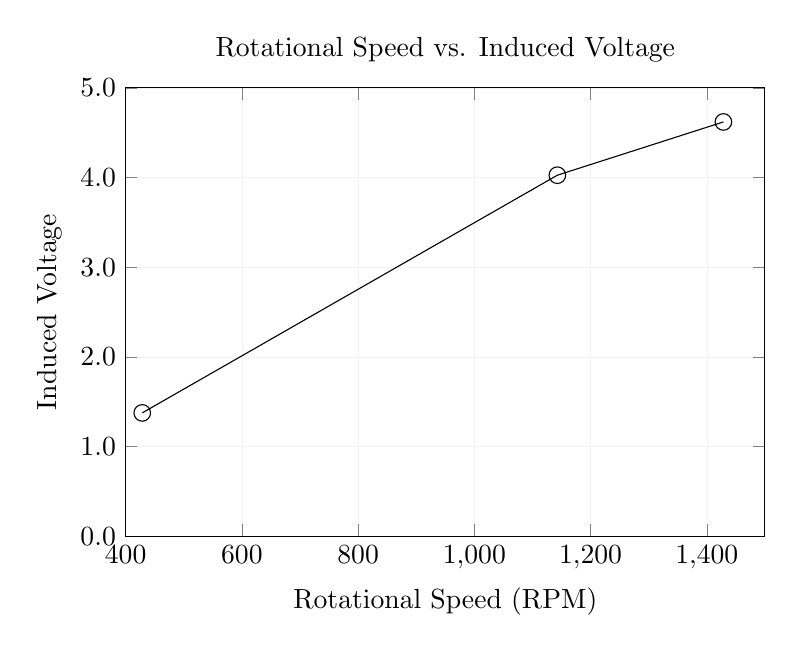
\begin{tikzpicture}
        \begin{axis}[
	    width=\textwidth,
            xlabel={Rotational Speed (RPM)},
            ylabel={Induced Voltage},
            title={Rotational Speed vs. Induced Voltage},
            grid=both,
            grid style={line width=.1pt, draw=gray!10},
            width=0.8\textwidth,
            height=0.6\textwidth,
            legend pos=north west,
            legend style={font=\footnotesize},
            mark size=3pt,
            xmin=400, xmax=1500,
            ymin=0, ymax=5,
            xtick={400,600,...,1400},
            ytick={0,1,2,3,4,5},
            y tick label style={
                /pgf/number format/.cd,
                fixed,
                fixed zerofill,
                precision=1,
                /tikz/.cd
            },
            x tick label style={
                /pgf/number format/.cd,
                fixed,
                fixed zerofill,
                precision=0,
                /tikz/.cd
            },
            ]
            
            \addplot[mark=o,mark size=3pt] coordinates {
                (428.5714286, 1.375)
		(1142.857143, 4.026)
		(1428.571429, 4.62)
            };
        \end{axis}
    \end{tikzpicture}
	\caption{Relationship between rotational speed and induced voltage for the generator}\label{fig:induction}
\end{figure}
We can see that as RPM increases induced voltage also increases, this is straightforward from Electromagnetic Induction. \\
We know that \[V=-N\frac{d\Phi}{dt},\] where \(\Phi\) is the magnetic flux. 
Also, \[\Phi=\mathbf{B}.\mathbf{S},\] where \(\mathbf{B}\) is the magnetic field density and \(\mathbf{S}\) is the surface area vector.\\
\begin{align}
	\text{Therefore, } V&=-N\frac{d}{dt}(\mathbf{B}.\mathbf{S})\\
	V&=-N\frac{d}{dt}(|B||S| Cos\omega t)\\
	V&=N|B||S|\omega Sin(\omega t)
\end{align}
Thus we get an expression for the Induced Voltage. If we look at this expression we can see that this induced voltage will be maximum when \(Sin(\omega t)\) is maximised. 
Thus, \begin{equation}
	V_{max}=2\pi f N |B||S|
\end{equation}

\section{Conclusion}
The series of experiments provided valuable insights into the fundamental
principles of DC motor manufacture and control. 
We learned about the physical structures of brushed and brushless DC motors. 
The hands-on experiences allowed for practical application of theoretical knowledge, reinforcing
concepts such as Electromagnetic Induction, Faraday's Law etc. 
We learned about all the different things that can influence motor rotation characteristics. 

\listoffigures
\listoftables

\end{document}
